\documentclass{beamer}
\usetheme{metropolis}
\usepackage{graphicx}
\usepackage{amsmath}
\usepackage{tcolorbox}
\title{Elementary Statistics: Math 080}
\author{Jordan Hanson}
\institute{Whittier College Department of Physics and Astronomy}

\begin{document}
\maketitle

\section{Summary}

\begin{frame}{Summary}
Unit 2 and 3
\begin{enumerate}
\item Central Limit Theorem: 7.1
\item Confidence Intervals and Hypothesis Testing
\begin{itemize}
\item Confidence intervals and data interpretation: 8.1 - 8.4
\item Rejecting the null hypothesis, types of error, underlying distributions: 9.1 - 9.3
\end{itemize}
\end{enumerate}
\end{frame}

\section{The Central Limit Theorem}

\begin{frame}{The Central Limit Theorem}
\begin{tcolorbox}[colback=orange!10,colframe=orange!100,title=The Central Limit Theorem]
\textbf{Central Limit Theorem:} Let X be a continuous random variable, with mean $\mu_x$ and standard deviation $\sigma_x$.  The average $\bar{x}$ of $n$ values of X is normally distributed like $N(\mu_x,\sigma_x/\sqrt{n})$.
\end{tcolorbox}
\end{frame}

\begin{frame}{The Central Limit Theorem}
\begin{figure}
\centering
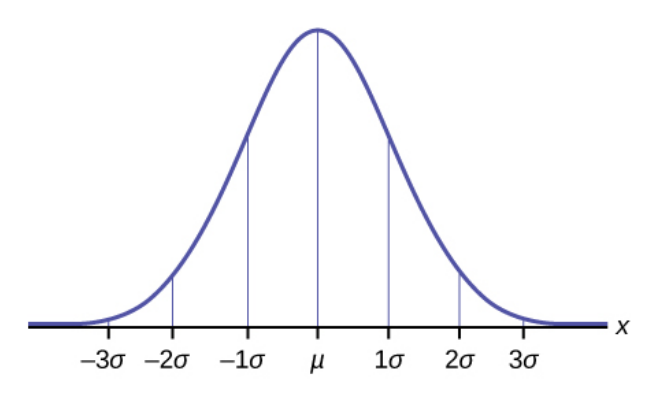
\includegraphics[width=0.5\textwidth]{figures/norm.png}
\caption{\label{fig:norm} The normal distribution about a mean $\mu$ with the units of standard deviations shown.}
\end{figure}
\textbf{Example:} An unknown distribution has a mean of $\mu = 90$ and a standard deviation of $\sigma = 15$. Samples of size $n = 25$ are drawn randomly from the population.  Find the probability that the \textit{sample mean} is between 87 and 93. \\ \vspace{1cm}
\end{frame}

\section{Interactive Questions}

\begin{frame}{Interactive Questions: Central Limit Theorem}
Suppose we take samples of size $n = 16$ from a large data set and compute the averages and standard deviations of the samples.  Suppose we repeat the whole process, but change $n = 100$.  Which of the following is true?
\begin{itemize}
\item A: The means of our samples will shift upwards by a factor of $100/16$.
\item B: The means of our samples will shift downwards by a factor of $100/16$.
\item C: The standard deviations of our samples will shift downwards by a factor of $\sqrt{100/16}$.
\item D: The standard deviations of our samples will shift upwards by a factor of $\sqrt{100/16}$.
\end{itemize}
\end{frame}

\begin{frame}{Interactive Questions: Central Limit Theorem}
Suppose we take samples of size $n = 100$ from a large data set that has mean $\mu$ and standard deviation $\sigma$, and compute the averages and standard deviations of the \textit{samples}.  Which of the following is true?
\begin{itemize}
\item A: Each standard deviation of each sample we collect will be $\sigma/10$.
\item B: The standard deviation of the means of our samples will be $\sigma/10$.
\item C: Each mean of each sample we collect will be $\mu/10$.
\item D: The mean of the means of our samples will be $\mu$.
\end{itemize}
\end{frame}

\section{Confidence Intervals}

\begin{frame}{Confidence Intervals}
Suppose we are attempting to measure a population parameter, such as the mean, $\mu$.  This is distinct from the \textit{sample mean,} $\bar{x}$, of a set of data $\left \lbrace x_i \right \rbrace$.
\begin{figure}
\centering
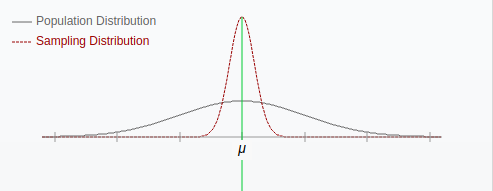
\includegraphics[width=0.85\textwidth]{figures/samples.png}
\caption{\label{fig:samp} Let the gray curve refer to a \textit{population} of data.  Let the red curve refer to the \textit{distribution of averages} we find if we repeatedly sample.  The standard deviation of the red curve is smaller because of the Central Limit Theorem: $\sigma_{\bar{x}} = \sigma_{pop}/\sqrt{n}$.}
\end{figure}
\end{frame}

\begin{frame}{Confidence Intervals}
\begin{figure}
\centering
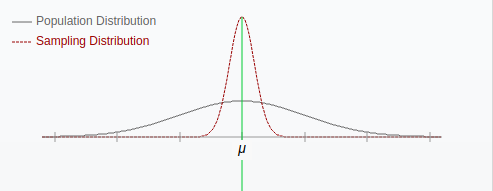
\includegraphics[width=0.85\textwidth]{figures/samples.png}
\caption{\label{fig:samp2} Suppose we decide to communicate the range in which the true mean $\mu$ falls, using our \textit{point estimates} $\bar{x}$.  How should we do that?}
\end{figure}

A good range: (Mean of $\bar{x}$ distribution minus two standard deviations), to (mean of $\bar{x}$ distribution plus two standard deviations).  \textbf{\alert{This interval has a 95 percent chance of containing $\mu$.}}
\end{frame}

\begin{frame}{Confidence Intervals}
\small
(Mean of $\bar{x} - 2s/\sqrt{n}$), to (Mean of $\bar{x} + 2s/\sqrt{n}$).  \textbf{\alert{This interval has a 90 percent chance of containing $\mu$.}} \\ 
\begin{itemize}
\item The error bound for the population mean (EBM) is the ``two standard deviations'' in this example, in which we know the population $\sigma$.
\item Recall the 68 - 95 - 99.7 rule, and how sample means are normally distributed regardless of the underlying distribution.
\item We choose the confidence level (CL), and construct the confidence interval for the given CL.
\item $\alpha = 1 -CL$, probability the confidence interval \textit{does not contain} $\mu$.
\end{itemize}
\textbf{Professor example, next slide.}
\end{frame}

\begin{frame}{Confidence Intervals}
\textbf{Professor example.} \\ \vspace{7cm}
\end{frame}

\section{PhET: Illustration of Confidence Intervals}

\begin{frame}{PhET: Confidence Intervals}
\small
Go to this link: \url{https://digitalfirst.bfwpub.com/stats_applet/stats_applet_4_ci.html}
\begin{enumerate}
\item Select a confidence level (CL) of 95 percent using the slide bar at left.
\item Set your sample size to 100.  The sample means will be distributed like $N(\mu,\sigma/\sqrt{n})$.  \alert{This example assumes we know $\sigma$, the population standard deviation, but we do not know the mean $\mu$.}
\item Hit the green Sample 25 button to collect 25 samples of size 100, to get 25 means.
\item How many of these means fall within two standard deviations $\sigma/\sqrt{100}$ (CL: 95 percent) of the true mean $\mu$?
\item Repeatedly hit Sample 25, and notice what happens to the percentage at left of sample means that fall within 2 $\sigma/\sqrt{100}$ of $\mu$.
\end{enumerate}
\end{frame}

\section{Interactive Questions}

\begin{frame}{Interactive Questions}
Suppose you wanted to measure the average age of inhabitants of a large neighborhood.  The population mean $\mu$ is unknown, but we can be reasonably certain that our sample standard deviations, $s_1$, $s_2$, ... are approximately $\sigma$, the standard deviation of the population.  So we know that the $\sigma_{age} = 20$ years.  Suppose we collect 100 samples of 16 people apiece.  This means the standard error in our mean $20/\sqrt{16} = 5$ years. \\
\begin{enumerate}
\item Suppose the mean of all our data is 70 years.  What is the EBM for two standard deviations in the mean?
\item How many of our samples should fall within 1 EBM of the true mean?
\end{enumerate}
\textbf{\alert{Solve via Breakout Rooms!  Go.}}
\end{frame}

\section{Hypothesis Testing}

\begin{frame}{Hypothesis Testing}
\begin{tcolorbox}[colback=orange!10,colframe=orange!100,title=The Null Hypothesis and Type I and II Errors]
Let the \textbf{null hypothesis} $H_0$ be a claim, true or false, about a population of data, and $H_a$ represent an alternative.  If samples from the data confirm $H_0$, then we accept $H_0$ as correct.  There are two potential errors: Type I and type II.  They are listed in Tab. \ref{tab:err}.  If $H_0$ and $H_a$ are \textit{complementary}, then rejecting $H_0$ confirms $H_a$.
\end{tcolorbox}
\begin{table}
\begin{tabular}{| c | c | c |}
\hline
& $H_0$ is True & $H_0$ is False \\ \hline
Do not reject $H_0$ & Correct & Type II Error \\ \hline
Reject $H_0$ & Type I Error & Correct \\ \hline
\end{tabular}
\caption{\label{tab:err} Summary of Type I and Type II errors.  The probability of a Type I error is $\alpha$, and the probability of a Type II is $\beta$.}
\end{table}
\end{frame}

\begin{frame}{Hypothesis Testing}
\textbf{Steps for rejection or confirmation of the null hypothesis:} assume underlying distribution is normal via the Central Limit Theorem.
\begin{enumerate}
\item The probability of a Type I error is $\alpha$, and the probability of a Type II is $\beta$.  \textit{Choose a value of $\alpha$ that is appropriate.}
\item Collect the sample of data.  Calculate the mean (or other point estimate of a population parameter).
\item Determine the probability $p$ that the mean occurred randomly, given the underlying distribution.
\item If $p < \alpha$, reject $H_0$.  If $p \geq \alpha$, accept $H_0$.
\end{enumerate}
\end{frame}

\begin{frame}{Hypothesis Testing}
\textbf{Steps for rejection or confirmation of the null hypothesis:} assume underlying distribution is normal via the Central Limit Theorem.\\ \vspace{0.5cm}
\textbf{Example procedure:} \\ \vspace{5cm}
\end{frame}

\begin{frame}[fragile]{Hypothesis Testing}
\begin{figure}
\centering
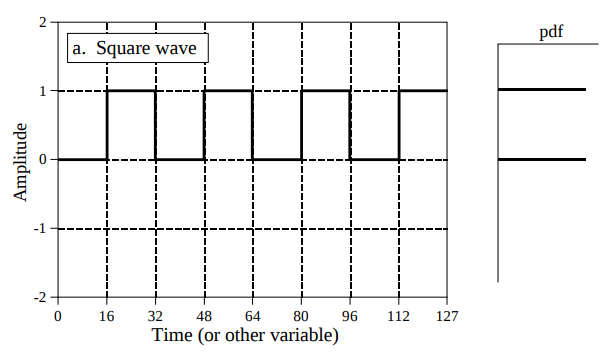
\includegraphics[width=0.7\textwidth]{figures/squarepdf.png}
\caption{\label{fig:squarepdf} The square-wave signal spends equal time at 0.0 and 1.0, and the probability density function reflects that.}
\end{figure}
\end{frame}

\begin{frame}[fragile]{Hypothesis Testing}
\begin{figure}
\centering
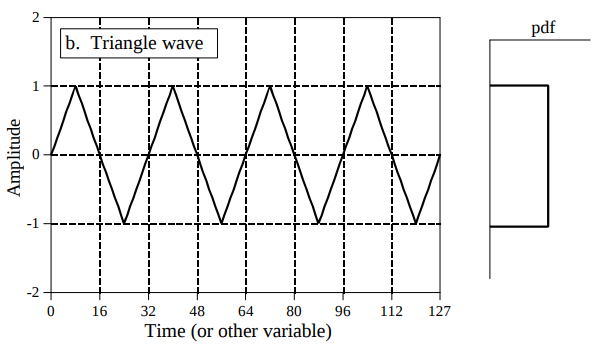
\includegraphics[width=0.7\textwidth]{figures/trianglepdf.png}
\caption{\label{fig:trianglepdf} The triangle-wave signal spends equal time at all values \textit{between} 0.0 and 1.0, and the probability density function reflects that.}
\end{figure}
\end{frame}

\begin{frame}[fragile]{Hypothesis Testing}
\begin{figure}
\centering
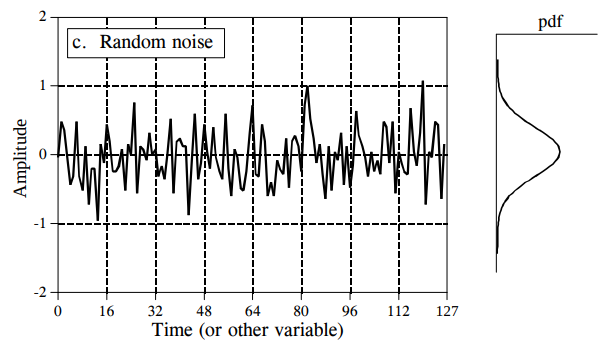
\includegraphics[width=0.7\textwidth]{figures/randnpdf.png}
\caption{\label{fig:randnpdf} The random noise \textit{usually} spends time near 0.0, but rarely it fluctuates to larger values.}
\end{figure}
\end{frame}

\begin{frame}{Hypothesis Testing}
\textbf{Example procedure for signals hidden in noise:} \\ \vspace{5cm}
\end{frame}

\begin{frame}{Hypothesis Testing}
When a new drug is created, the pharmaceutical company must subject it to testing before receiving the necessary
permission from the Food and Drug Administration (FDA) to market the drug. Suppose the null hypothesis is ``the drug creates harmful side effects in 5 percent of patients.'' What is the Type I Error?
\begin{itemize}
\item A: To claim the drug harms fewer than 5 percent of patients, and it harms fewer than 5 percent of patients.
\item B: To claim the drug harms fewer than 5 percent of patients, and it harms more than 5 percent of patients.
\item C: To claim the drug harms more than 5 percent of patients, and it harms fewer than 5 percent of patients.
\item D: To claim the drug harms more than 5 percent of patients, and it harms more than 5 percent of patients.
\end{itemize}
\end{frame}

\begin{frame}{Hypothesis Testing}
When a new drug is created, the pharmaceutical company must subject it to testing before receiving the necessary
permission from the Food and Drug Administration (FDA) to market the drug. Suppose the null hypothesis is ``the drug creates harmful side effects in 5 percent of patients.'' What is the Type II Error?
\begin{itemize}
\item A: To claim the drug harms fewer than 5 percent of patients, and it harms fewer than 5 percent of patients.
\item B: To claim the drug harms fewer than 5 percent of patients, and it harms more than 5 percent of patients.
\item C: To claim the drug harms more than 5 percent of patients, and it harms fewer than 5 percent of patients.
\item D: To claim the drug harms more than 5 percent of patients, and it harms more than 5 percent of patients.
\end{itemize}
\end{frame}

\begin{frame}[fragile]{Hypothesis Testing}
\small
Suppose we are presented with the data in Fig. \ref{fig:randnpdf2}.  $H_0$: there will be no outliers more than three standard deviations from the mean in 256 days.  Do you accept $H_0$?  Why or why not?  What is your chosen $\alpha$?
\begin{figure}
\centering
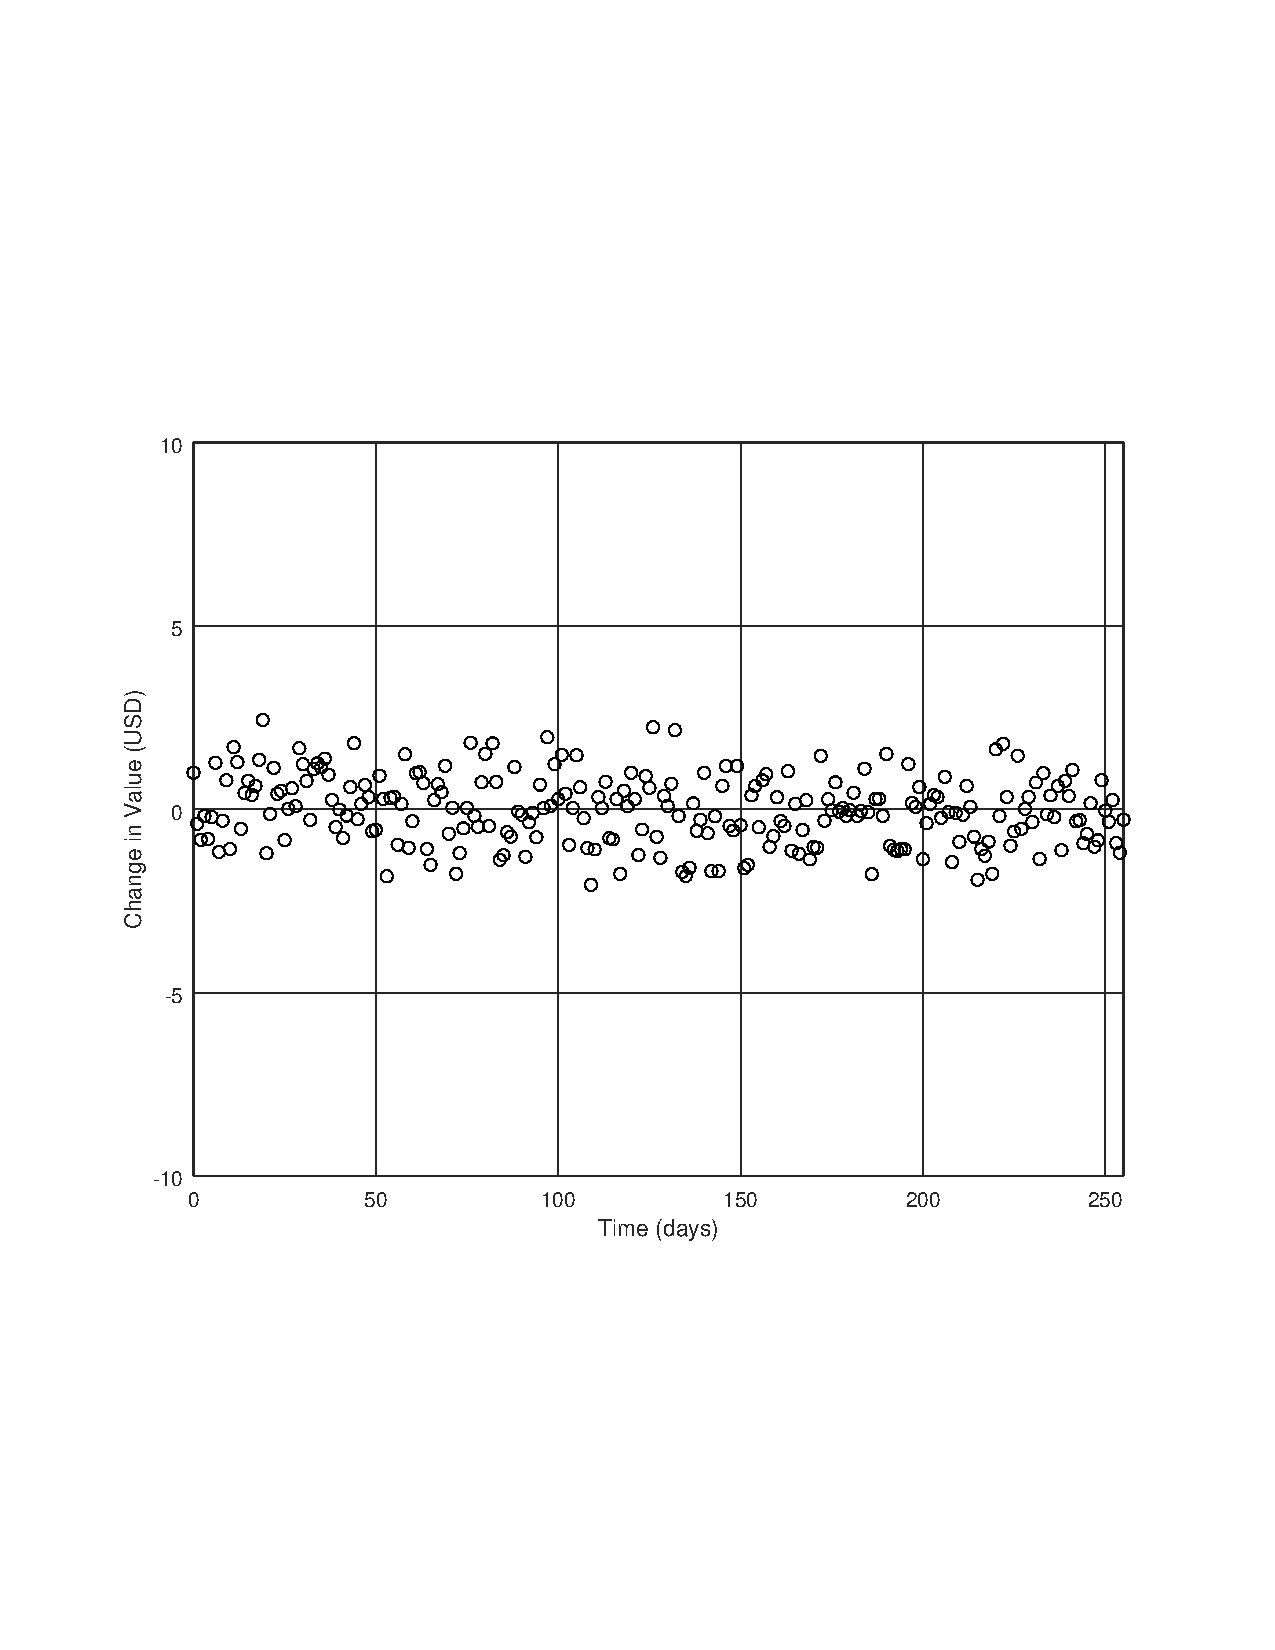
\includegraphics[width=0.65\textwidth,trim=0cm 7cm 0cm 5cm,clip=true]{figures/randn.pdf}
\caption{\label{fig:randnpdf2} The change in the account, in USD, versus time, in days.}
\end{figure}
\end{frame}

\section{Conclusion}

\begin{frame}{Summary}
Unit 2 and 3
\begin{enumerate}
\item Central Limit Theorem: 7.1
\item Confidence Intervals and Hypothesis Testing
\begin{itemize}
\item Confidence intervals and data interpretation: 8.1 - 8.4
\item Rejecting the null hypothesis, types of error, underlying distributions: 9.1 - 9.3
\end{itemize}
\end{enumerate}
\end{frame}

\end{document}